\begin{frame}{First-Order: Computing the Step Response}
    Assume initial rest.
    \begin{columns}[T,totalwidth=\textwidth]
        \begin{column}{0.5\textwidth}
            \begin{align*}
                \frac{dv_C(t)}{dt} + \frac{1}{RC}v_C(t) &= \frac{1}{RC}v_I(t).\\
                \frac{dv_C(t)}{dt} + \frac{1}{RC}v_C(t) &= \frac{1}{RC}u(t)
            \end{align*}
            \begin{align*}
                sV_C(s) + \frac{1}{RC}V_C(s) &= \frac{1}{RC}\frac{1}{s}\\
                V_C(s) &= \frac{\frac{1}{RC}}{s(s+ \frac{1}{RC})}\\
                &= \frac{1}{s}  - \frac{1}{s+ \frac{1}{RC}}
            \end{align*}
        \end{column}
        \begin{column}{0.5\textwidth}
            \begin{align*}
                v_c(t) &= u(t) - e^{-\frac{1}{RC}t}u(t)\\
                v_c(t) &= \left(1 - e^{-\frac{1}{RC}t}\right)u(t)
            \end{align*}
            Plot with $RC=1$:
            \begin{center}
                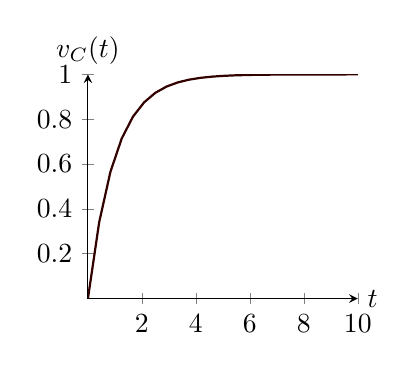
\begin{tikzpicture}
\def\R{1}
\def\C{1}
\begin{axis}
	[
		scale=0.5,
		xlabel = {$t$},
		ylabel = {$v_C(t)$},
		 axis lines=middle,
		xlabel style={at=(current axis.right of origin), anchor=west},
		ylabel style={at=(current axis.above origin), anchor=south},		
	]
	\addplot [red!20!black, thick, domain=0:10] {(1- e^(-x/(\R*\C)))};
\end{axis}

\end{tikzpicture} 
            \end{center}            
        \end{column}
    \end{columns}
\end{frame}